\documentclass[t]{beamer}
% number subsubsections and put them in the table of contents...
\setcounter{tocdepth}{3}
\setcounter{secnumdepth}{3}

\newcommand{\notimp}{\emph{Status:} Not yet implemented.}

% algorithm2e package settings...

\SetInd{1mm}{2mm}
\SetVlineSkip{.5mm}
\SetKw{Break}{break}
\SetKw{Assert}{assert}
\SetKw{Integer}{Integer}
\SetKw{Array}{array}
\SetKw{Of}{of}
\SetKwFor{Procedure}{procedure}{is}{end procedure}
\SetKwInOut{Uses}{uses}
\SetKwInOut{Invariant}{invariant}

% Type/font styles...
\newcommand{\upsty}[1]{\textup{\textsf{#1}}}
\newcommand{\setsty}[1]{\textup{\textsf{\textcolor{blue}{#1}}}}
\newcommand{\code}[1]{\texttt{\textcolor{blue}{#1}}}
\newcommand{\ct}[1]{\texttt{#1}}

% Theorem environments...
\newtheorem{theorem}{Theorem}
\theoremstyle{definition}
\newtheorem{definition}{Definition}[subsection]

% Symbols...
\renewcommand{\implies}{\Rightarrow}
\newcommand{\ra}{\rightarrow}
\newcommand{\B}{\mathbb{B}}
\newcommand{\N}{\mathbb{N}}
\newcommand{\lb}{\texttt{\char`\{}}
\newcommand{\rb}{\texttt{\char`\}}}
\newcommand{\U}{\texttt{\char`\_}}
%\newcommand{\U}{{\ttfamily\symbol{'137}}}
\newcommand{\UU}{\U\U}

% Static notions...
\newcommand{\rootscope}{\setsty{root}} % root static scope
\newcommand{\start}{\setsty{start}} % start location $l_0$
\newcommand{\Var}{\setsty{Var}} % set of all variables
\newcommand{\bool}{\setsty{bool}} % boolean type
\newcommand{\proc}{\setsty{proc}} % process reference type
\newcommand{\Val}{\setsty{Val}} % set of all values
\newcommand{\vtype}{\setsty{vtype}} % type of variable
\newcommand{\etype}{\setsty{etype}} % type of expression
\newcommand{\Type}{\setsty{Type}} % set of all types
\newcommand{\Expr}{\setsty{Expr}} % set of all expressions
\newcommand{\Eval}{\setsty{Eval}} % set of all valuations on variables
\newcommand{\eval}{\setsty{eval}} % evaluation of an expression
\newcommand{\sparent}{\setsty{sparent}} % parent of a static scope
\newcommand{\dparent}{\setsty{dparent}} % parent of a dynamic scope
\newcommand{\fscope}{\setsty{fscope}} % scope of a function
\newcommand{\lscope}{\setsty{lscope}} % scope of a location
\newcommand{\static}{\setsty{static}} % static scope associated to a dynamic one
\newcommand{\stack}{\setsty{stack}} % call stack
\newcommand{\vars}{\setsty{vars}} % variables declared in a scope
\newcommand{\ancestors}{\setsty{ancestors}} % as in tree
\newcommand{\descendants}{\setsty{descendants}} % as in tree
\newcommand{\returntype}{\setsty{returnType}} % function's return type
\newcommand{\numparams}{\setsty{numParams}} % number of params for a func.
\newcommand{\params}{\setsty{params}} % sequence of formal parameters
\newcommand{\void}{\setsty{void}} % type for func. returning nothing
\newcommand{\Loc}{\setsty{Loc}} % locations in function's trans. sys.
\newcommand{\Func}{\mathcal{F}} % set of function symbols
\newcommand{\true}{\textit{true}} % boolean value true
\newcommand{\false}{\textit{false}} % boolean value false
\newcommand{\default}{\setsty{default}} % default value of type
\newcommand{\len}{\setsty{length}} % length of sequence
\newcommand{\func}{\setsty{func}} % function a static scope belongs to

% Dynamic notions...
\newcommand{\fnode}{\setsty{fnode}} % function node of dyscope
\newcommand{\State}{\setsty{State}} % set of all states of model
\newcommand{\deval}{\setsty{deval}} % valuation on dyscope
\newcommand{\droot}{\setsty{droot}} % root dyscope
\newcommand{\Frame}{\setsty{Frame}} % set of activation frames

% Tables...
\newcommand{\notationtable}{%
  \begin{tabular}{lll}
    Symbol & Section & Meaning\\ \hline
    $\B$ & \S\ref{sec:notation} & \{\true,\false\}\\
    $\N$ & \S\ref{sec:notation} & \{0,1,2,\ldots\}\\
    $\ancestors$ & \S\ref{sec:notation} & set of ancestors of node in a tree (inclusive)\\
    $\descendants$ & \S\ref{sec:notation} & set of descendants of node
    in a tree (inclusive)\\
    $\len$ & \S\ref{sec:notation} & length of a sequence\\
    $\Var$ & \S\ref{sec:context} & the set of all variables\\
    $\bool$ & \S\ref{sec:context} & the boolean type\\
    $\proc$ & \S\ref{sec:context} & the process reference type\\
    $\Val$ & \S\ref{sec:context} & the set of all values\\
    $\Val_t$ & \S\ref{sec:context} & values of type $t$\\
    $\default_t$ & \S\ref{sec:context} & default value of type $t$\\
    $\vtype$ & \S\ref{sec:context} & function $\Var\ra\Type$ giving type of each variable\\
    $\Eval$ & \S\ref{sec:context} & set of all valuations on $\Var$\\
    $\Eval(V)$ & \S\ref{sec:state} & set of all valuations on variables in $V\subseteq\Var$\\
    $\Expr$ & \S\ref{sec:context} & set of typed expressions over $\Var$\\
    $\etype$ & \S\ref{sec:context} & $\Expr\ra\Type$, gives type of each expression\\
    $\eval$ & \S\ref{sec:context} & $\Expr\times\Eval\ra\Val$, the evaluation function\\
    $\mathcal{C}$ & \S\ref{sec:context} & a CIVL context\\
    $\Sigma$ & \S\ref{sec:scopes} & set of all static scopes\\
    $\rootscope$ & \S\ref{sec:scopes} & the root scope (member of $\Sigma$)\\
    $\sparent$ & \S\ref{sec:scopes} & $\Sigma\setminus\{\rootscope\}\ra\Sigma$, parent function in static scope tree\\
    $\vars$ & \S\ref{sec:scopes} & $\Sigma\ra 2^{\Var}$, specifies variables declared in scope\\
    $\Lambda$ & \S\ref{sec:scopes} & a lexical scope system\\
    $\void$ & \S\ref{sec:functions} & type used for function that does not return  a value\\
    $\Type'$ & \S\ref{sec:functions} & $\Type\cup\{\void\}$\\
    $\Func$ & \S\ref{sec:functions} & set of function symbols\\
    $\fscope$ & \S\ref{sec:functions} & $\Func\ra\Sigma\setminus\{\rootscope\}$, gives function scope of each function\\
    $\returntype$ & \S\ref{sec:functions} & $\Func\ra\Type'$, gives return type of each function\\
%    $\numparams$ & \S\ref{sec:functions} & $\Func\ra\N$, gives number of inputs for each function\\
    $\params$ & \S\ref{sec:functions} & $\Func\ra\Var^*$, formal
    parameter sequence for $f\in\Func$\\
    $f_0$ & \S\ref{sec:functions} & the root function (member of
    $\mathcal{F}$)\\
    $\func$ & \S\ref{sec:functions} & $\Sigma\ra\Func$, function to
    which scope belongs\\
    $\Loc_f$ & \S\ref{sec:gts} & set of locations for $f\in\Func$\\
    $\lscope_f$ & \S\ref{sec:gts} & $\Loc_f\ra\Sigma$, gives scope of each location for $f\in\Func$\\
    $\start_f$ & \S\ref{sec:gts} & start location for $f\in\Func$ (member of $\Loc_f$)\\
    $T_f$ & \S\ref{sec:gts} & set of guarded transitions for $f\in\Func$\\
  \end{tabular}
}


% CIVL-C keywords

\newcommand{\cckey}{\$}
\newcommand{\cc}[1]{\mbox{\texttt{\cckey{}#1}}}
\newcommand{\cabstract}{\cc{abstract}}
\newcommand{\ccontains}{\cc{contains}}
\newcommand{\ccopy}{\cc{copy}}
\newcommand{\cproc}{\cc{proc}}
\newcommand{\cprocdefined}{\cc{proc{\U}defined}}
\newcommand{\cprocNull}{\cc{proc{\U}null}}
\newcommand{\cself}{\cc{self}}
\newcommand{\cinput}{\cc{input}}
\newcommand{\coutput}{\cc{output}}
\newcommand{\cspawn}{\cc{spawn}}
\newcommand{\cwait}{\cc{wait}}
\newcommand{\cwaitall}{\cc{waitall}}
\newcommand{\cassert}{\cc{assert}}
\newcommand{\ctrue}{\cc{true}}
\newcommand{\cfalse}{\cc{false}}
\newcommand{\cassume}{\cc{assume}}
\newcommand{\catom}{\cc{atom}}
\newcommand{\catomic}{\cc{atomic}}
\newcommand{\cwhen}{\cc{when}}
\newcommand{\cchoose}{\cc{choose}}
\newcommand{\cchooseint}{\cc{choose{\U}int}}
\newcommand{\cinvariant}{\cc{invariant}}
\newcommand{\crequires}{\cc{requires}}
\newcommand{\censures}{\cc{ensures}}
\newcommand{\cexit}{\cc{exit}}
\newcommand{\cresult}{\cc{result}}
\newcommand{\cat}{\texttt{@}}
\newcommand{\ccollective}{\cc{collective}}
\newcommand{\cequals}{\cc{equals}}
\newcommand{\cfor}{\cc{for}}
\newcommand{\cparfor}{\cc{parfor}}

%\newcommand{\cheap}{\cc{heap}}
\newcommand{\cscope}{\cc{scope}}
\newcommand{\cscopedefined}{\cc{scope{\U}defined}}
\newcommand{\cscopeof}{\cc{scopeof}}
\newcommand{\cscopeparent}{\cc{scope{\U}parent}}
\newcommand{\cscoperoot}{\cc{root}}
\newcommand{\chere}{\cc{here}}
\newcommand{\cregion}{\cc{region}}
\newcommand{\cmalloc}{\cc{malloc}}
\newcommand{\cfree}{\cc{free}}

\newcommand{\cbundle}{\cc{bundle}}
\newcommand{\cbundlesize}{\cc{bundle{\U}size}}
\newcommand{\cbundlepack}{\cc{bundle{\U}pack}}
\newcommand{\cbundleunpack}{\cc{bundle{\U}unpack}}
\newcommand{\cbundleunpackapply}{\cc{bundle{\U}unpack{\U}apply}}

\newcommand{\cmessage}{\cc{message}}
\newcommand{\cmessagepack}{\cc{message{\U}pack}}
\newcommand{\cmessagesource}{\cc{message{\U}source}}
\newcommand{\cmessagetag}{\cc{message{\U}tag}}
\newcommand{\cmessagedest}{\cc{message{\U}dest}}
\newcommand{\cmessagesize}{\cc{message{\U}size}}
\newcommand{\cmessageunpack}{\cc{message{\U}unpack}}


\newcommand{\ccomm}{\cc{comm}}
\newcommand{\ccommcreate}{\cc{comm{\U}create}}
\newcommand{\cgcomm}{\cc{gcomm}}
\newcommand{\cgcommcreate}{\cc{gcomm{\U}create}}

\newcommand{\cbarrier}{\cc{barrier}}
\newcommand{\cgbarrier}{\cc{gbarrier}}
\newcommand{\cgbarriercreate}{\cc{gbarrier{\U}create}}
\newcommand{\cbarriercreate}{\cc{barrier{\U}create}}
\newcommand{\cbarriercall}{\cc{barrier{\U}call}}
\newcommand{\cgbarrierdestroy}{\cc{gbarrier{\U}destroy}}
\newcommand{\cbarrierdestroy}{\cc{barrier{\U}destroy}}

\newcommand{\cseqinit}{\cc{seq{\U}init}}
\newcommand{\cseqlen}{\cc{seq{\U}length}}
\newcommand{\cseqinsert}{\cc{seq{\U}insert}}
\newcommand{\cseqrm}{\cc{seq{\U}remove}}

\newcommand{\cforall}{\cc{forall}}
\newcommand{\cexists}{\cc{exists}}
\newcommand{\cimplies}{\ct{=>}}

\newcommand{\crange}{\cc{range}}
\newcommand{\cdomain}{\cc{domain}}
\newcommand{\cdomainof}[1]{\cc{domain}\ct{(}#1\ct{)}}

% version information
\newcommand{\version}{v1.3}
\newcommand{\versiondate}{2015-07-23}

\foot{CIVL Tutorial}
\date{\today}
\title{{\huge\bf CIVL}\\
  Concurrency Intermediate Verification Language\\ \ \\
  Tutorial}

\begin{document}

\begin{frame}[plain]
  \titlepage
\end{frame}


\section{CIVL User Tutorial}

\begin{frame}{What is CIVL?}
  CIVL is \ldots
  \begin{enumerate}
  \item \ldots a programming language, \alert{CIVL-C}
    \begin{itemize}
    \item based on subset of C
    \item extensions for concurrency, naming of scopes
    \end{itemize}
  \item \ldots a suite of tools for analyzing CIVL-C programs
    \begin{itemize}
    \item running + dynamic checking
    \item model checking
    \item static analyses (coming)
    \end{itemize}
  \item \ldots a set of translators from common programming
    language/concurrency API combinations to CIVL-C
    \begin{itemize}
    \item coming
    \end{itemize}
  \end{enumerate}
\end{frame}

\begin{frame}{Some CIVL-C primitives}
  \begin{tabular}{ll}
    \cproc & the process type \\
    \cself & the evaluating process (constant of type \cproc) \\
    \cscope & the scope type \\
    \cinput & type qualifier declaring variable to be a program input \\
    \coutput & type qualifier declaring variable to be a program output \\
    \cspawn & create a new process running procedure \\
    \cwait & wait for a process to terminate \\
    \cassert & check something holds \\
    \ctrue & boolean value true, used in assertions \\
    \cfalse & boolean value false, used in assertions \\
    \cassume & assume something holds \\
    \cwhen & guarded statement \\
    \cchoose & nondeterministic choice statement \\
    \cchooseint & nondeterministic choice of integer
  \end{tabular}
\end{frame}

\begin{frame}{CIVL Command line tools}
  \begin{itemize}
  \item \code{civl run filename}
    \begin{itemize}
    \item run the CIVL program making nondeterministic choices randomly
    \item \code{-seed=LONG} : use this random seed (reproducible)
    \end{itemize}
  \item \code{civl verify filename}
    \begin{itemize}
    \item explore reachable state space, checking properties at each state
      \begin{itemize}
      \item absence of deadlock, assertion violations, division by $0$,
        invalid pointer dereference, out of bounds array access, \ldots
      \end{itemize}
    \item may specify bounds using \cinput{} variables and command line
      \begin{itemize}
      \item \code{-inputX=value}
      \end{itemize}
    \item \code{-errorBound=INT} specifies maximum number of errors that
      will be logged before quitting
    \end{itemize}
  \item \code{civl replay}
    \begin{itemize}
    \item  if a violation was found during \code{verify}, its trace
      is saved to a file; this will run the trace
    \item \code{-id=INT} can be used to specify the ID of the trace if more than one
    \item \code{-trace=tracefile} can be used to specify the exact filename 
      containing trace
    \end{itemize}
  \end{itemize}  
\end{frame}

\begin{frame}[containsverbatim]{Example: \code{adder.cvl}}

  \begin{tabular}[t]{l|l}
    \begin{minipage}[t]{.45\textwidth}\scriptsize
\begin{verbatim}
#include <civlc.h>

$input int B;
$input int N;
$assume 0<=N && N<=B;
$input double a[N];

double adderSeq(double *p, int n) {
  double s = 0.0;
  
  for (int i = 0; i < n; i++)
    s += p[i]; 
  return s;
}

double adderPar(double *p, int n) {
  double s = 0.0;
  _Bool mutex = 0;
  $proc workers[n];

  void worker(int i) {
    double t;
\end{verbatim}
    \end{minipage}
    &
    \begin{minipage}[t]{.45\textwidth}\scriptsize
\begin{verbatim}
    $when (mutex == 0) mutex = 1;
    t = s;
    t += p[i];
    s = t;
    mutex = 0;
  }
  
  for (int j = 0; j < n; j++)
    workers[j] = $spawn worker(j);
  for (int j = 0; j < n; j++)
    $wait workers[j];
  return s;
}

void main() {
  double seq = adderSeq(&a[0], N);
  double par = adderPar(&a[0], N);

  $assert seq == par;
}
\end{verbatim}
    \end{minipage}
  \end{tabular}
\end{frame}

\begin{frame}[containsverbatim]{Verifying \code{adder.cvl}}

  \begin{small}
\begin{verbatim}
concurrency$ civl verify -inputB=5 adder.cvl
CIVL v0.8 of 2014-03-03 -- http://vsl.cis.udel.edu/civl

=================== Stats ===================
   validCalls          : 2801
   proverCalls         : 27
   memory (bytes)      : 128974848
   time (s)            : 4.25
   maxProcs            : 6
   statesInstantiated  : 4103
   statesSaved         : 777
   statesSeen          : 767
   statesMatched       : 72
   steps               : 1090
   transitions         : 838

The standard properties hold for all executions.
\end{verbatim}
  \end{small}
\end{frame}

\begin{frame}{Download and Installation}
  \begin{enumerate}
  \item Get a Java 7 VM.
  \item Go to \url{http://vsl.cis.udel.edu/civl}
  \item Navigate to downloads, \emph{latest stable release}.
  \item Download version corresponding to your platform.
    \begin{itemize}
    \item for now, pre-compiled versions for OS X and linux (32- and 64-bit)
    \item other platforms must build from source
    \end{itemize}
  \item Unpack and move resulting directory \texttt{CIVL-\textit{tag}}
    under \texttt{/opt}.
  \item Download the VSL dependencies archive.
    \begin{itemize}
    \item contains a number of pre-compiled open source libraries used by CIVL
    \item \url{http://vsl.cis.udel.edu/tools/vsl\_depend}
    \end{itemize}
  \item Unpack and move resulting directory \texttt{vsl} under \texttt{/opt}.
  \item Put \texttt{/opt/CIVL-\textit{tag}/bin/civl} in your path.
    \begin{itemize}
    \item however you want: move it, symlink, \ldots
    \end{itemize}
  \end{enumerate}

  \alert{Note:} You can put \texttt{vsl} and \texttt{CIVL-\textit{tag}}
  in any directories (not just \texttt{/opt}).  Just edit script \texttt{civl}
  to use the new paths.
\end{frame}

\begin{frame}[containsverbatim]{Test your installation}

  From command line \ldots

\begin{verbatim}
concurrency$ civl
CIVL v0.8 of 2014-03-03 -- http://vsl.cis.udel.edu/civl
Missing command
Type "civl help" for command line syntax.

concurrency$ civl help
...
\end{verbatim}

Copy \texttt{/opt/CIVL-\textit{tag}/examples/concurrency/adder.cvl}
to your working directory and try

\begin{verbatim}
    civl verify -inputB=5 adder.cvl
\end{verbatim}
\end{frame}

\begin{frame}{What features are inherited from C?}
  \begin{itemize}
  \item most syntax
  \item types
    \begin{itemize}
    \item \texttt{{\U}Bool} $\ra$ $\{0,1\}$
    \item \texttt{int}, \texttt{long}, \texttt{short}, \ldots $\ra$ $\Z$
    \item \texttt{double}, \texttt{float}, \ldots $\ra$ $\R$
    \item structure, array, pointer, and function types
    \end{itemize}
  \item expressions
    \begin{itemize}
    \item addition, multiplication, division, subtraction, unary minus (\code{+}, 
      \code{*}, \code{/}, \code{-})
    \item integer division (\code{/}) and modulus (\code{\%})
    \item pointer dereference (\code{*}), address-of (\code{\&})
    \item array subscript (\code{[...]})
    \item structure navigation (\code{.})
    \item logical and (\code{\&\&}), or (\code{||}), not (\code{!})
    \item \code{==}, \code{!=}, \code{<}, \code{>}, \code{<=}, \code{>=}
    \item pointer addition (\code{+}) and subtraction (\code{-})
    \item \code{++}, \code{--}
    \item \alert{no bit-wise operations} for now
    \end{itemize}
  \end{itemize}
\end{frame}

\begin{frame}{Inherited from C, cont.}
  \begin{itemize}
  \item statements
    \begin{itemize}
    \item no-op, labeled-statement, compound-statement
    \item assignments (\code{=}, \code{+=}, \code{-=}, \ldots)
    \item function call
    \item \code{if}\ldots\code{else}
    \item \code{goto}, \code{while}, \code{do}, \code{for},
      \code{switch}, \code{break}
    \end{itemize}
  \item procedure (function) prototypes and definitions
  \item \code{typedef}
  \item preprocessing directives
  \end{itemize}
\end{frame}

\begin{frame}{New features}
  \begin{itemize}
  \item functions can be declared in any scope
  \item concurrency primitives
    \begin{itemize}
    \item spawning processes: \code{\cproc\ p = \cspawn\ f();}
    \item waiting for a process to terminate: \code{\cwait\ p;}
    \item guarded commands: \code{\cwhen (x>0) c=1;}
    \end{itemize}
  \item nondeterministic choice: \code{\cchoose ...}
  \item first-class scope objects: \code{\cscope\ s;}
  \item other primitives useful for verification
    \begin{itemize}
    \item input qualifier, assert, assume, procedure contracts
    \end{itemize}
  \item library-level constructs supporting message-passing, \ldots
  \end{itemize}
\end{frame}

\begin{frame}[containsverbatim]{CIVL-C encoding of Dijkstra's Dining Philosophers}
  \begin{scriptsize}
\begin{verbatim}
#include <civlc.h>

$input int B; // upper bound on number of philosophers
$input int n; // number of philosophers
$assume 2<=n && n<=B;
_Bool forks[n]; // Each fork will be on the table (0) or in a hand (1). 

void dine(int id) {
  int left = id;
  int right = (id + 1) % n;

  while (1) {
    $when (forks[left] == 0) forks[left] = 1;
    $when (forks[right] == 0) forks[right] = 1;
    forks[right] = 0;
    forks[left] = 0;
  }
}

void main() {
  for (int i = 0; i < n; i++) forks[i] = 0;
  for (int i = 0; i < n; i++) $spawn dine(i);
}
\end{verbatim}
  \end{scriptsize}
\end{frame}

\begin{frame}{Example Illustrating Scopes and Processes}
  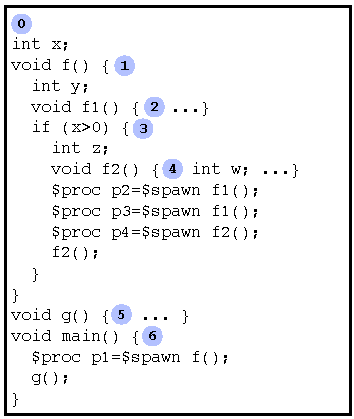
\includegraphics[scale=1.1]{scopeCodeExample}
\end{frame}

\begin{frame}{Static scope tree and a state for example}
  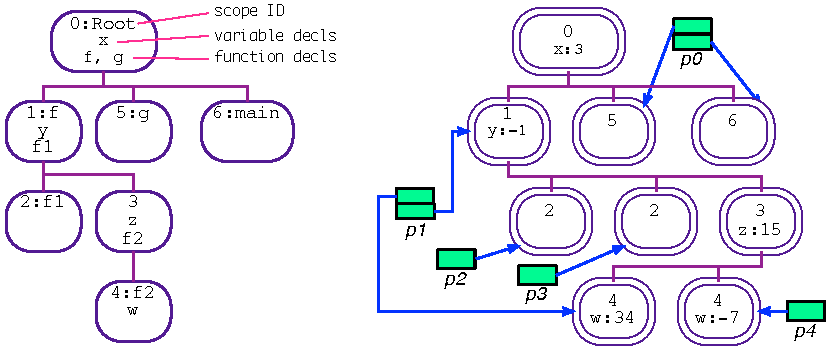
\includegraphics[scale=.85]{scopeStateExample}
\end{frame}

\begin{frame}{Scopes and processes: key points}
\begin{itemize}
\item In any state, there is a mapping from the dyscope tree to the
  static scope tree which maps a dyscope to the static scope of which
  it is an instance.  This mapping is a \alert{tree homomorphism},
  i.e., if dyscope $u$ is a child of dyscope $v$, then the static
  scope corresponding to $u$ is a child of the static scope
  corresponding to $v$.
\item A static scope may have any number of instances, including 0.
\item Dynamic scopes are created when control enters the corresponding
  static scope; they disappear from the state when they become
  unreachable.  A dyscope $v$ is \alert{reachable} if some process has a
  frame pointing to a dyscope $u$ and there is a path from $u$ up to
  $v$ that follows the parent edges in the dyscope tree.
\item Processes are created when functions are spawned; they disappear
  from the state when their stack becomes empty (either because the
  process terminates normally or invokes the \alert{\emph{exit}}
  system function).
\end{itemize}
\end{frame}

\begin{frame}{Bundles}
  \begin{itemize}
  \item there is a special \cbundle{} type
  \item represents a ``chunk'' of data
    \begin{itemize}
    \item actually a sequence of elements of one type
    \end{itemize}
  \item can make one bundle from a sequence of ints, another from a
    sequence of floats
    \begin{itemize}
    \item both bundles have the same type: \cbundle
    \end{itemize}
  \item if \texttt{b} has type \cbundle, \texttt{b} can hold either
    bundle
  \end{itemize}
\end{frame}

\begin{frame}[containsverbatim]{Bundle API}
\begin{verbatim}
/* Creates a bundle from the memory region specified
 * by ptr and size, copying the data into the new
 * bundle */
$bundle $bundle_pack(void *ptr, int size);

/* Returns the size (number of bytes) of the bundle */
int $bundle_size($bundle b);

/* Copies the data out of the bundle into the
 * region specified */
void $bundle_unpack($bundle bundle, void *ptr);
\end{verbatim}
\end{frame}

\begin{frame}[containsverbatim]{The \cscope{} type}
  \begin{itemize}
  \item an object of type $\cscope$ is a reference to a dynamic scope
  \item it may be thought of as a ``dynamic scope ID''
    \begin{itemize}
    \item but it is not an integer and cannot be converted to an
      integer
    \end{itemize}
  \item operations
    \begin{itemize}
    \item \code{==}, \code{!=}
    \item \code{s<t} : \code{s} is a proper sub-scope of \code{t}
    \item \code{<=}, \code{>}, \code{>=}
    \item \code{s+t}
      \begin{itemize}
      \item the lowest common ancestor (LCA) of \code{s} and \code{t}
        in dyscope tree
      \item the smallest dyscope containing both \code{s} and \code{t}
      \end{itemize}
    \item \code{scopeof(lhs)}
      \begin{itemize}
      \item the scope containing object specified by the
        left-hand-side expression
      \end{itemize}
    \end{itemize}
  \item constants
    \begin{itemize}
    \item \chere: this dynamic scope
    \item \cscoperoot: the root dynamic scope
    \end{itemize}
  \item functions
    \begin{itemize}
    \item \verb!$scope $scope_parent($scope s);!
    \end{itemize}
  \end{itemize}
\end{frame}

\begin{frame}[containsverbatim]{\cscopeof{} example: all assertions hold}
  \begin{small}
\begin{verbatim}
{
  $scope s1 = $here;
  int x;
  double a[10];

  {
    $scope s2 = $here;
    int *p = &x;
    double *q = &a[4];

    assert($scopeof(x)==s1);
    assert($scopeof(p)==s2);
    assert($scopeof(*p)==s1);
    assert($scopeof(a)==s1);
    assert($scopeof(a[5])==s1);
    assert($scopeof(q)==s2);
    assert($scopeof(*q)==s1);
  }
}  
\end{verbatim}
  \end{small}
\end{frame}

\begin{frame}[containsverbatim]{Statements}
  The usual C statements are supported:
  \begin{itemize}
  \item \emph{no-op} (\ct{;})
  \item expression statements (\ct{e;})
  \item labeled statements, including \ct{case} and \ct{default} labels
    (\ct{l: s})
  \item \emph{for} (\ct{for (init; cond; inc) s}), \emph{while} 
    (\ct{while (cond) s}) and \emph{do} (\ct{do s while (cond)})
    loops
  \item compound statements (\lb \ct{s1;s2;} \ldots \rb)
  \item \texttt{if} and \verb!if! \ldots \verb!else!
  \item \verb!goto!
  \item \verb!switch!
  \item \verb!break!
  \item \verb!continue!
  \item \verb!return!
  \end{itemize}
\end{frame}

\begin{frame}[containsverbatim]{Guarded commands: \cwhen}
  A guarded command is encoded using a \cwhen{} statement:
\begin{verbatim}
  $when (expr) stmt;
\end{verbatim}
  \begin{itemize}
  \item all statements have a guard, either implicit or explicit
  \item for most statements, the guard is \emph{true}
  \item the \cwhen{} statement allows one to attach an explicit guard
    to a statement
  \item when \texttt{expr} is \emph{true}, the statement is
    \alert{enabled}, otherwise it is \alert{disabled}
  \item a disabled statement is \alert{blocked}---it will not
    be scheduled for execution
  \item when it is enabled, it may execute by
    moving control to the \texttt{stmt} and executing the first atomic
    action in the \texttt{stmt}.
  \end{itemize}
\end{frame}

\begin{frame}{Guards, cont.}
  \begin{itemize}
  \item if \texttt{stmt} itself has a non-trivial guard:
    \begin{itemize}
    \item the guard of the \cwhen{} statement is the conjunction of
      \texttt{expr} and the guard of \texttt{stmt}
    \end{itemize}
  \item the evaluation of \texttt{expr} and the first atomic action of
    \texttt{stmt} occur as a single atomic action
  \item  there is no guarantee that execution of \texttt{stmt}
    will continue atomically if it contains more than one atomic
    action
    \begin{itemize}
    \item i.e., other processes may be scheduled
    \end{itemize}
  \end{itemize}
\end{frame}

\begin{frame}[containsverbatim]{Guard examples}
\begin{verbatim}
  $when (s>0) s--;
\end{verbatim}
  \begin{itemize}
  \item blocks until \texttt{s} is positive then decrements \texttt{s}
  \item execution of \texttt{s--} is guaranteed to take place
    in an environment in which \texttt{s} is positive
  \end{itemize}

\begin{verbatim}
  $when (s>0) {s--; t++}
\end{verbatim}
  \begin{itemize}
  \item execution of \texttt{s--} must happen when \texttt{s>0}
  \item between \texttt{s--} and \texttt{t++}, other processes may
    execute
  \end{itemize}

\begin{verbatim}
  $when (s>0) $when (t>0) x=y*t;
\end{verbatim}
  \begin{itemize}
  \item blocks until both \texttt{x} and \texttt{t} are positive then
    executes the assignment
  \item equivalent to:
\begin{verbatim}
  $when (s>0 && t>0) x=y*t;
\end{verbatim}
  \end{itemize}
\end{frame}

\begin{frame}[containsverbatim]{Nondeterministic selection statement: \cchoose}
\begin{verbatim}
  $choose {
    stmt1;
    stmt2;
    ...
    default: stmt
  }
\end{verbatim}

  \begin{itemize}
  \item  the \texttt{default} clause is optional
  \item the guards of the statements are evaluated and among those that are
    \emph{true}, one is chosen nondeterministically and executed
  \item if none are \emph{true} and the \texttt{default} clause is
    present, it is chosen
  \item the \texttt{default} clause will only be selected if all
    guards are \emph{false}
  \item if no \texttt{default} clause and
    all guards are \emph{false}, the statement blocks
  \item implicit
    guard of \cchoose{} statement without \texttt{default} clause is
    the disjunction of the guards of its sub-statements
  \item implicit guard of \cchoose{} statement with a default
    clause is \emph{true}.
  \end{itemize}
\end{frame}

\begin{frame}[containsverbatim]{Using \cchoose{} to encode a
    transition system}
\begin{verbatim}
  l1: $choose {
    $when (x>0) {x--; goto l2;}
    $when (x==0) {y=1; goto l3;}
    default: {z=1; goto l4;}
  }
  l2: $choose {
    ...
  }
  l3: $choose {
    ...
  }
\end{verbatim}
\end{frame}


\begin{frame}[containsverbatim]{Nondeterministic choice of integer: \cchooseint}
  The system function \cchooseint{} has the following signature:

\begin{verbatim}
  int $choose_int(int n);
\end{verbatim}

  This function takes as input a positive integer \texttt{n} and
  nondeterministicaly returns an integer in the range
  $[0,\texttt{n}-1]$.
\end{frame}

\begin{frame}{The process type: \cproc}
  \begin{itemize}
  \item a primitive object type and functions like any other primitive
    C type (e.g., \texttt{int})
  \item an object of this type refers to a
    process
  \item it can be thought of as a process ID
    \begin{itemize}
    \item but it is not an integer and cannot be cast to one
    \item it is analogous to the $\cscope$ type for dynamic scopes
    \end{itemize}
  \item certain expressions take an argument of \cproc{} type and some return
    something of \cproc{} type
  \end{itemize}
\end{frame}

\begin{frame}{Spawning a new process: \cspawn}
  \begin{itemize}
  \item a \emph{spawn} expression is an expression with side-effects
  \item spawns a new process and returns a reference to the new
    process
    \begin{itemize}
    \item an object of type \cproc
    \end{itemize}
  \item syntax is the same as a procedure invocation with the keyword
    \cspawn{} inserted in front:
    \begin{itemize}
    \item \code{\cspawn\ f(expr1, ..., exprn)}
    \end{itemize}
  \item typically the returned value is assigned to a variable, e.g.:
    \begin{itemize}
    \item \code{\cproc\ p = \cspawn f(i);}
    \end{itemize}
  \item if \texttt{f} returns a value, that value is ignored
  \end{itemize}
\end{frame}

\begin{frame}{Waiting for another process to terminate: \cwait}

  The system function $\cwait$ has signature

  \begin{center}
    \code{void\ \cwait(\cproc\ p);}
  \end{center}

  \begin{itemize}
  \item when invoked, this function will not return until the process
    referenced by \ct{p} has terminated.
  \item note that $p$ can be any
    expression of type \cproc{}, not just a variable.
  \end{itemize}
\end{frame}

\begin{frame}{Terminating a process immediately: \cexit}
  \begin{itemize}
  \item this function takes no arguments
  \item it causes the calling process to terminate immediately,
    regardless of the state of its call stack
  \item \code{void\ \cexit(void);}
  \end{itemize}
\end{frame}



\begin{frame}<0>{Scope-parameterized pointers}
  \begin{itemize}
  \item a declaration of the form \code{\cscope\ s;} assigns the name
    \code{s} to the containing scope
    \begin{itemize}
    \item what you can do with \code{s} is very limited
    \item cannot be assigned, passed as parameter
    \end{itemize}
  \item \code{int *<s> p;}
    \begin{itemize}
    \item declares \code{p} to have type ``pointer-to-\code{int}-in-\code{s}''
    \item \code{p} can only hold a pointer to an object in scope \code{s}
    \end{itemize}
  \item $s_1\leq s_2$ $\implies$
    \textit{pointer-to-$T$-in-$s_1$} \alert{is a subtype of}
    \textit{pointer-to-$T$-in-$s_2$}
  \item the type \textit{pointer-to-$T$} (\code{T*}) is shorthand for
    \textit{pointer-to-$T$-in-$s_0$} (\code{T*<\(s_0\)>}), where $s_0$
    is the \alert{root scope}
  \item \code{\&x} returns a pointer to the declaration scope of \code{x}
    \begin{itemize}
    \item scope of \code{\&a[i]} is the scope of \code{\&a}
    \item scope of \code{\&r.f} is the scope of \code{\&r}
    \end{itemize}
  \end{itemize}
\end{frame}

\begin{frame}<0>[containsverbatim]{Pointer safety}
  \begin{itemize}
  \item for a CIVL-C program to be \alert{statically type-safe},
    for all assignments, the type of the right-hand side must be a subtype
    of that of the left-hand side
  \item static type-safety can be checked statically
  \end{itemize}
  
  Example:
  
  \begin{mycbox}{7cm}
\begin{verbatim}
  {
    $scope s1;
    double x;
    {
      $scope s2;
      double a[N];
      double *<s1> p = &x; // OK
      double *<s2> q = &a[0]; // OK
      
      p = &a[1]; // OK
      q = &x; // static type error
    }
  }
\end{verbatim}
  \end{mycbox}
\end{frame}

\begin{frame}<0>[containsverbatim]{Scope-parameterized functions}

  A function declaration or definition may be parameterized by any number
  of \alert{formal scope parameters}.   Example:

  \begin{mycbox}{7cm}
\begin{verbatim}
  <s> int *<s> f(int *<s> p);
\end{verbatim}
  \end{mycbox}

  declares $f$ to be a function which, for any scope $s$, takes a
  \emph{pointer-to-\texttt{int}-in-$s$} and returns a
  \emph{pointer-to-\texttt{int}-in-$s$}.

\end{frame}

\begin{frame}<0>{Further ideas}
  \begin{itemize}
  \item scope-parameterized \alert{typedefs} and \alert{structs}
  \item \alert{heap} type (can have ``a heap in every scope'')
    \begin{itemize}
    \item \texttt{malloc} and \texttt{free} adjusted to take reference to heap
    \end{itemize}
  \item a \alert{bundle type}
    \begin{itemize}
    \item wrap up any contiguous region of memory into an object of bundle type
    \item functions to \alert{pack} and \alert{unpack} bundles
    \item useful for many abstractions, e.g., messages
    \end{itemize}
  \item set of functions and types supporting \alert{message-passing}
  \item see Trac Wiki and \code{civlc.h}
  \end{itemize}
\end{frame}

\begin{frame}[containsverbatim]{Message Passing example: \code{ring.cvl}}

\begin{verbatim}
/* Create nprocs processes.  Have them exchange data
 * in a cycle.  Commandline example:
 *     civl verify -inputNPROCS=3 ring.cvl -simplify=false
 */
#include<civlc.h>
#include "mp_root.cvh"

void MPI_Process (int rank) {
#include "mp_proc.cvh"

  double x=rank, y;

  send(&x, 1, (rank+1)%NPROCS, 0);
  recv(&y, 1, (rank+NPROCS-1)%NPROCS, 0);
  $assert y==(rank+NPROCS-1)%NPROCS;
}
\end{verbatim}
\end{frame}

\begin{frame}[containsverbatim]{File \code{mp{\U}root.cvh}}
  \scriptsize
\begin{verbatim}
$input int NPROCS;
$proc __procs[NPROCS];
_Bool __start = 0;
$comm MPI_COMM_WORLD;

void MPI_Process (int rank);

void init() {
  for (int i=0; i<NPROCS; i++)
    __procs[i] = $spawn MPI_Process(i);
  MPI_COMM_WORLD = $comm_create(NPROCS, __procs);
  __start=1;
}

void finalize() {
  for (int i=0; i<NPROCS; i++)
    $wait __procs[i];
}

void main() {
  init();
  finalize();
}
\end{verbatim}
\end{frame}

\begin{frame}[containsverbatim]{File \code{mp{\U}proc.cvh}}
  \scriptsize
\begin{verbatim}
  void send(void *buf, int count, int dest, int tag) {
    $message out = $message_pack(rank, dest, tag, buf, count*sizeof(double));
    $comm_enqueue(&MPI_COMM_WORLD, out);
  }

  void recv(void *buf, int count, int source, int tag) {
    $message in = $comm_dequeue(&MPI_COMM_WORLD, source, rank, tag);
    $message_unpack(in, buf, count*sizeof(double));
  }

  $when (__start);
\end{verbatim}
\end{frame}

\section{CIVL Developer Tutorial}

\begin{frame}{VSL Projects: Uses Relation}

  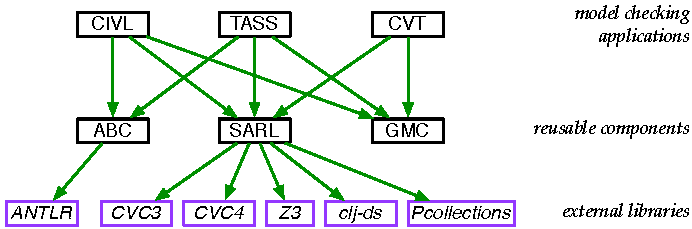
\includegraphics{vsl_projects}

  \begin{itemize}
  \item reusable components
    \begin{itemize}
    \item ABC: A Better C compiler?  ANTLR-Based C compiler?
    \item SARL: Symbolic Algebra \& Reasoning Library
    \item GMC: Generic Model Checking utilities
      \begin{itemize}
      \item DFS, command line interface, trace saving/replay, error
        logging, random simulation
      \end{itemize}
    \end{itemize}
  \item model checking applications
    \begin{itemize}
    \item CIVL: Concurrency Intermediate Verification Language
    \item TASS: Toolkit for Accurate Scientific Software (C+MPI)
    \item CVT: Chapel Verification Tool
    \end{itemize}
  \end{itemize}

\end{frame}

\begin{frame}{Engineering}

  \begin{itemize}
  \item all of the VSL software is in Java
  \item try to maintain coding standards
  \item clear module boundaries with interfaces
  \end{itemize}
  
  
  \begin{center}
    \begin{tabular}{|ll|}
      \hline
      Web page & \url{http://vsl.cis.udel.edu/civl}\\
      Subversion & \url{svn://vsl.cis.udel.edu/civl}\\
      Trac repository & \url{https://vsl.cis.udel.edu/trac/civl}\\
      Automated build/test & \url{http://vsl.cis.udel.edu/civl/test}\\
      \hline
    \end{tabular}
  \end{center}

  \begin{itemize}
  \item replace \texttt{civl} with \texttt{sarl}, \texttt{abc}, \texttt{gmc}, or
    \texttt{tass}
  \end{itemize}

  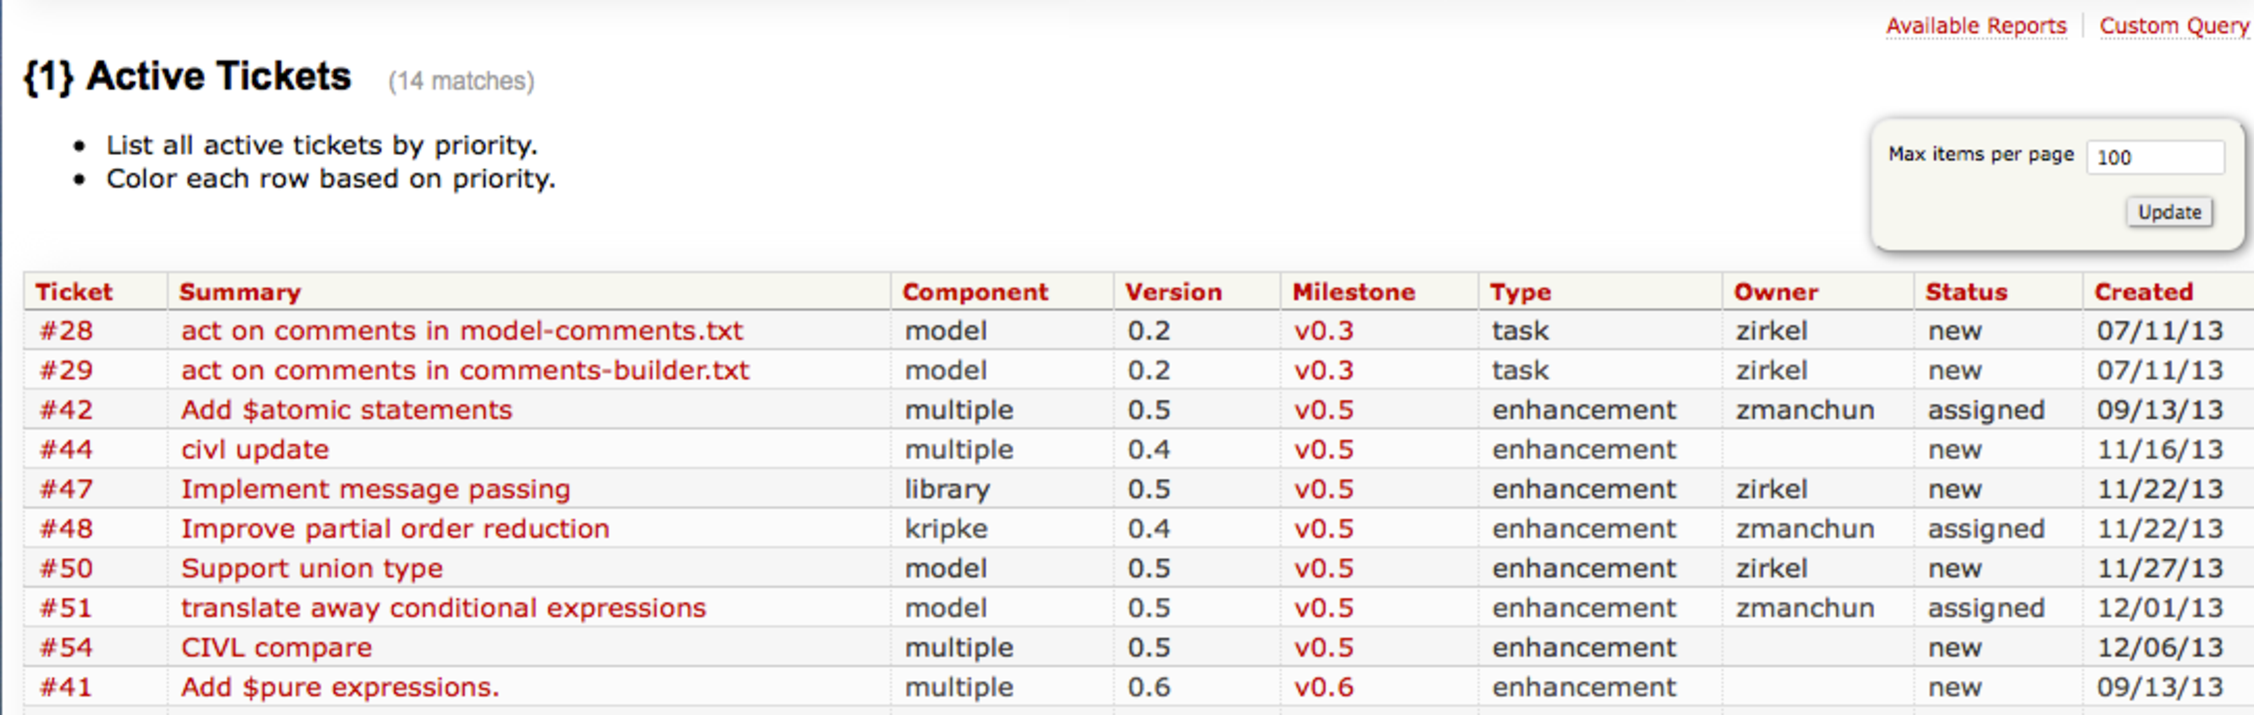
\includegraphics[scale=.3]{civl-trac.pdf}
  
\end{frame}

\begin{frame}{Civl Test Directory}
  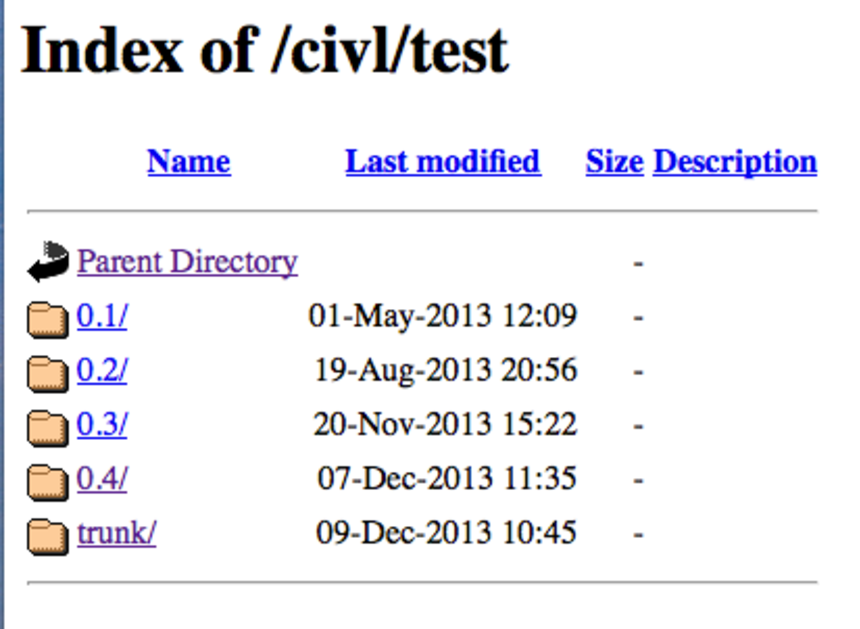
\includegraphics[scale=.35]{civlTestDir}
  
  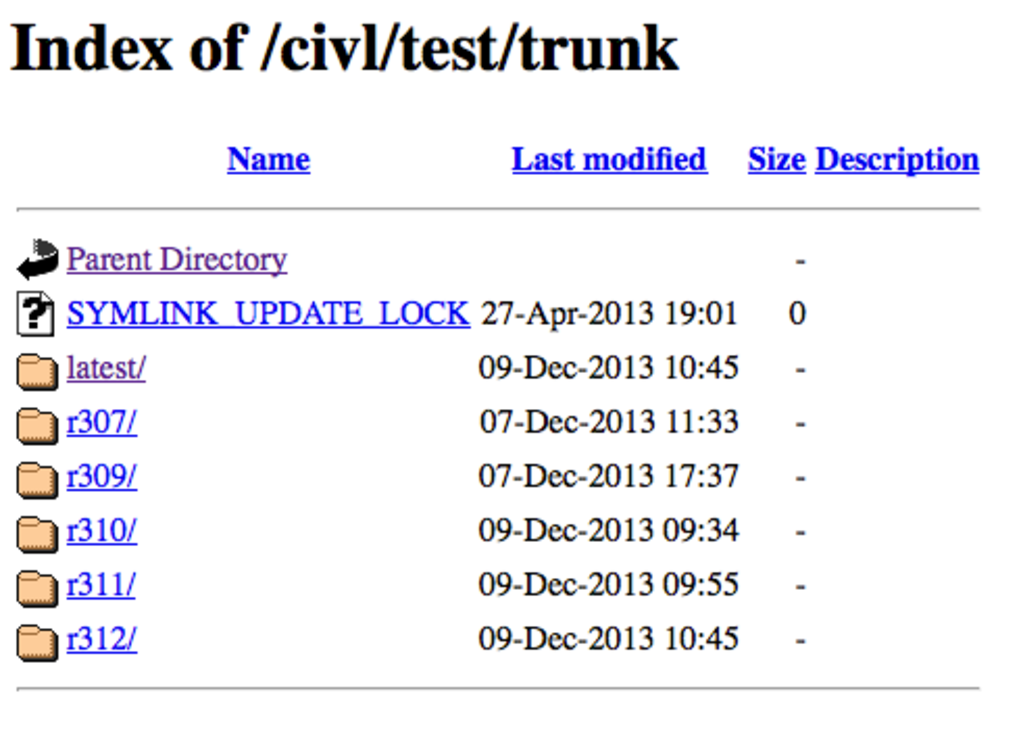
\includegraphics[scale=.35]{civlTestTrunkDir}
\end{frame}

\begin{frame}{CIVL Test Directory: Latest (unstable) Release}
  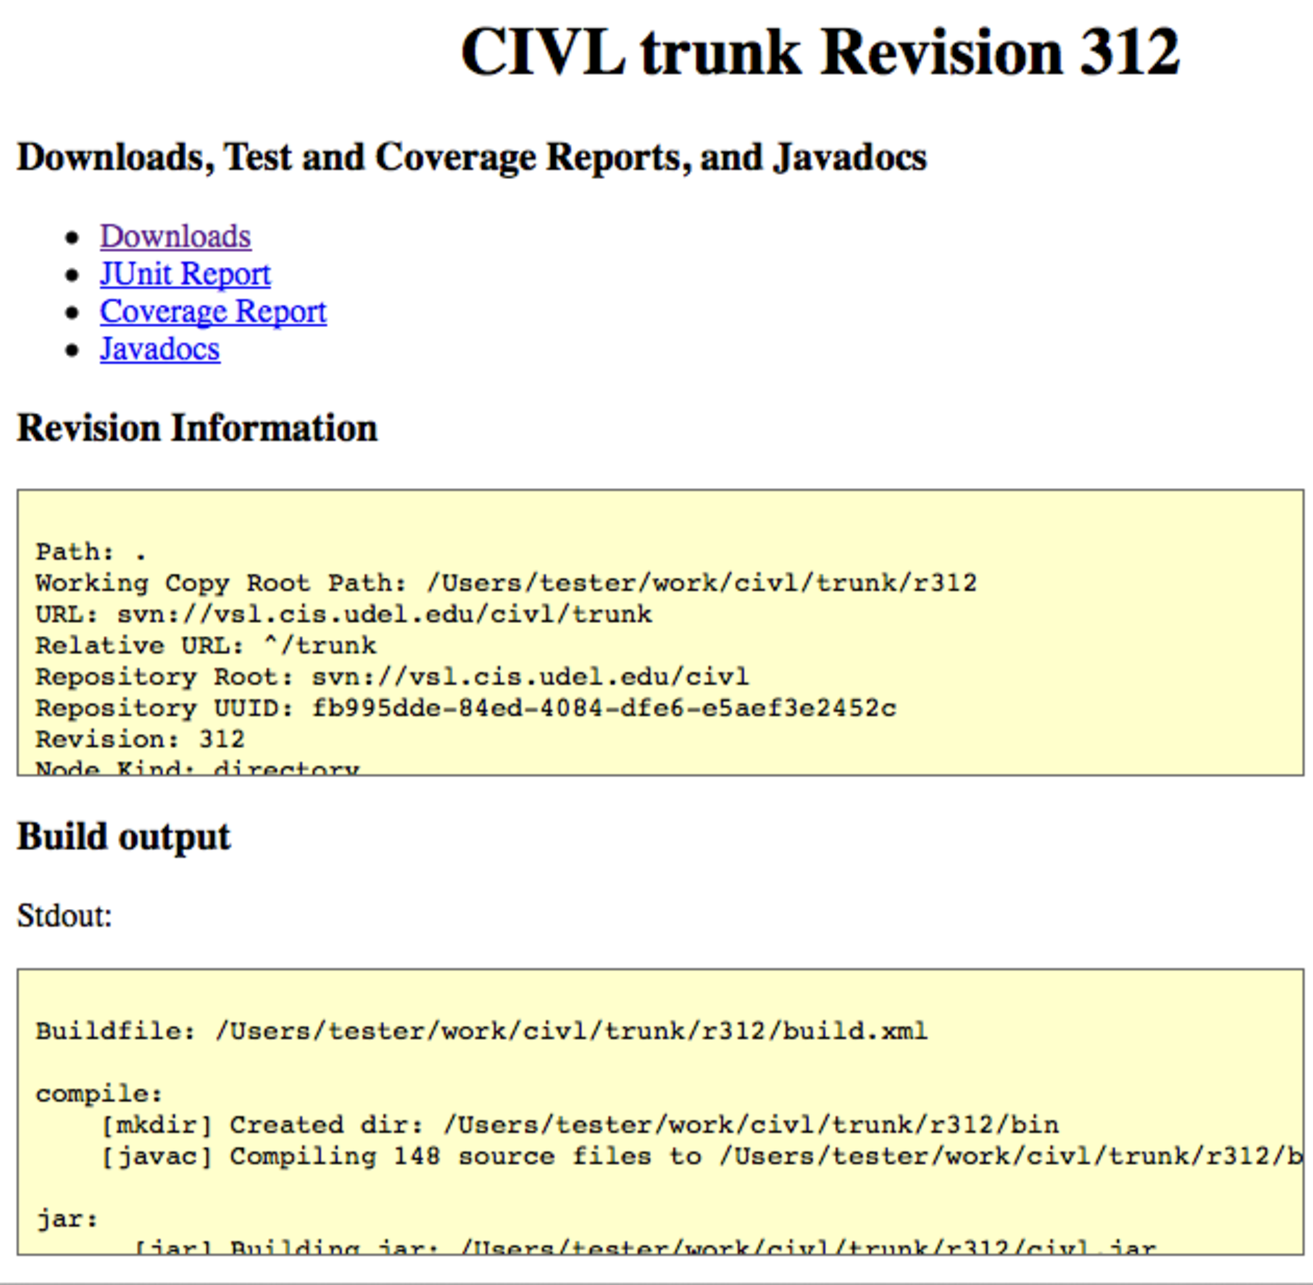
\includegraphics[scale=.35]{civlTestTrunkLatest}
\end{frame}


\begin{frame}{Automated Build \& Test Script}

  \begin{center}
    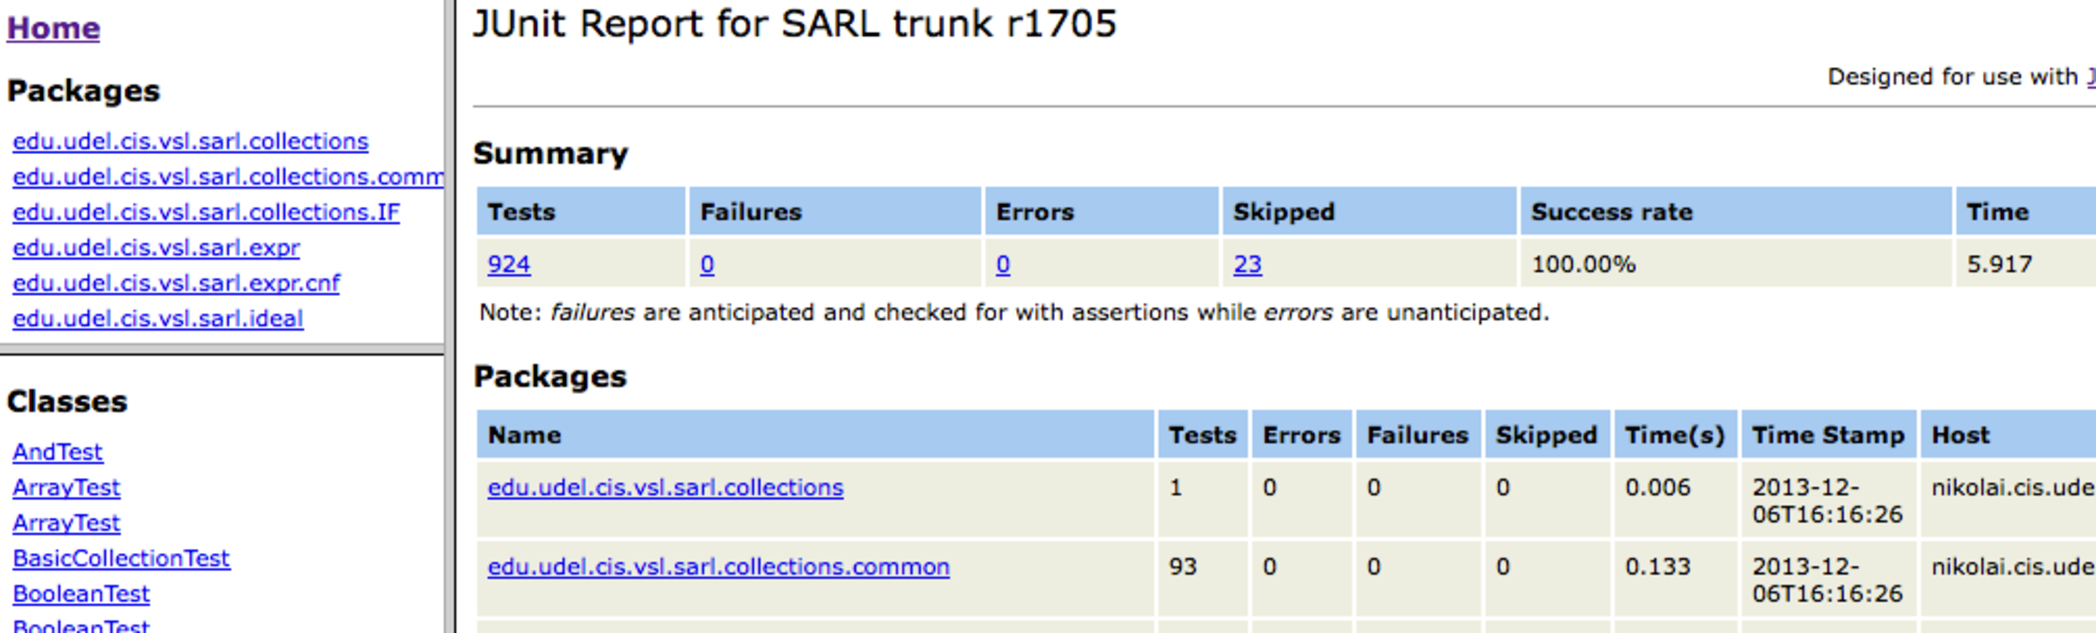
\includegraphics[scale=.3]{sarl-junit.pdf}
  \end{center}

  For each project \ldots
  \begin{itemize}
  \item script is run after each commit
  \item one directory for each \alert{branch} and \alert{trunk}
    \begin{itemize}
    \item one subdirectory for each revision, up to some bounded history
    \end{itemize}
  \item compiles all code and displays results
  \item runs JUnit test suite and displays results
  \item runs Jacoco coverage anaysis and displays results
  \item generates javadocs
  \end{itemize}
\end{frame}

\begin{frame}{Coverage Analysis Results}
  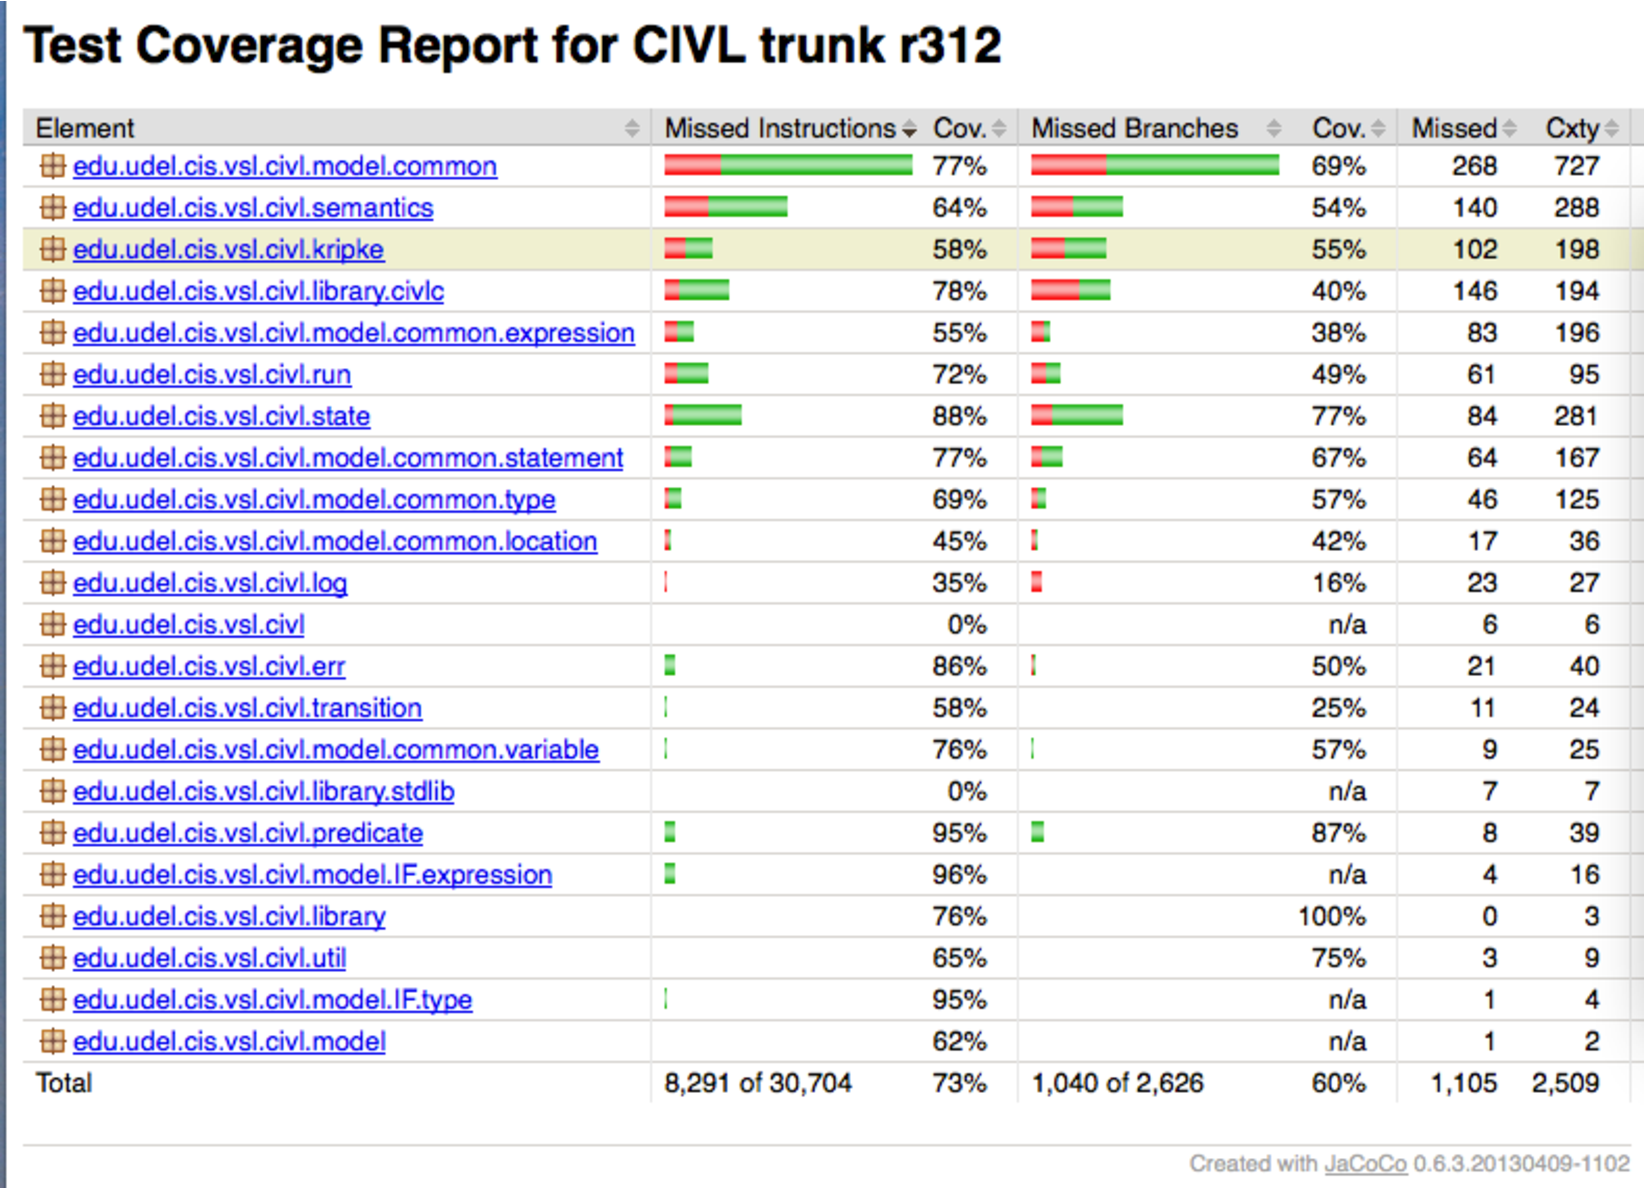
\includegraphics[scale=.4]{civlCoverage}
\end{frame}

\begin{frame}{Developer Eclipse Set-up}
  \begin{enumerate}
  \item Download vsl dependencies archive from
    \url{http://vsl.cis.udel.edu/tools/vsl_depend}
  \item Download and install Eclipse IDE for Java EE Developers
    \begin{itemize}
    \item version Kepler or later
    \end{itemize}
  \item Install Apache Ant if you don't have it
  \item Install an Eclipse SVN plugin (such as Subversive)
  \item Create class path variable \texttt{VSL}:
    \begin{itemize}
    \item Preferences$\ra$Java$\ra$Build Path$\ra$ClassPath Variables
    \item select ``New'' and create a classpath variable \texttt{VSL}
    \item specify its value to be \texttt{/opt/vsl}
    \end{itemize}
  \item Create string variable \texttt{vsl{\U}lib}:
    \begin{itemize}
    \item Preferences$\ra$Run/Debug$\ra$String Substitution$\ra$New
    \item define an entry \texttt{vsl{\U}lib}
    \item set its value to be \texttt{/opt/vsl/lib}
    \end{itemize}
  \end{enumerate}
\end{frame}

\begin{frame}{Check out and install ABC}
  \begin{enumerate}
  \item Check out ABC Eclipse project 
    \begin{itemize}
    \item ``New Project\ldots from SVN''
    \item SVN repository: \url{svn://vsl.cis.udel.edu/abc}
    \item Navigate and select \texttt{trunk} from within archive
    \item Check out project using all default options
    \end{itemize}
  \item Build using Ant
    \begin{itemize}
    \item right-click on \texttt{build.xml}
    \item Choose ``Run as Ant build''
    \item Clean project
    \end{itemize}
  \item test the build
    \begin{itemize}
    \item select Run$\ra$Run Configurations\ldots
    \item ceate a new JUnit 4 configuration called ``ABC Tests''
    \item select ``Run all tests in the selected project\ldots''
    \item navigate and select the \texttt{test} folder in the ABC project
    \item under the Arguments tab, type \texttt{-ea} into the VM arguments field
    \item click ``Run'' to run the tests
    \end{itemize}
  \end{enumerate}
\end{frame}

\begin{frame}{Check out and install GMC}
  \begin{enumerate}
  \item Check out GMC Eclipse project 
    \begin{itemize}
    \item ``New Project\ldots from SVN''
    \item SVN repository: \url{svn://vsl.cis.udel.edu/gmc}
    \item Navigate and select \texttt{trunk} from within archive
    \item Check out project using all default options
    \end{itemize}
  \item test the build
    \begin{itemize}
    \item select Run$\ra$Run Configurations\ldots
    \item ceate a new JUnit 4 configuration called ``GMC Tests''
    \item select ``Run all tests in the selected project\ldots''
    \item navigate and select the \texttt{test} folder in the GMC project
    \item under the Arguments tab, type \texttt{-ea} into the VM arguments field
    \item click ``Run'' to run the tests
    \end{itemize}
  \end{enumerate}
\end{frame}

\begin{frame}{Check out and install SARL}
  \begin{enumerate}
  \item Check out SARL Eclipse project 
    \begin{itemize}
    \item ``New Project\ldots from SVN''
    \item SVN repository: \url{svn://vsl.cis.udel.edu/sarl}
    \item Navigate and select \texttt{trunk} from within archive
    \item Check out project using all default options
    \end{itemize}
  \item test the build
    \begin{itemize}
    \item select Run$\ra$Run Configurations\ldots
    \item ceate a new JUnit 4 configuration called ``SARL Tests''
    \item select ``Run all tests in the selected project\ldots''
    \item navigate and select the \texttt{test} folder in the SARL project
    \item under Arguments tab, type \texttt{-ea} into the VM arguments field
    \item under Environment tab, create an entry
      \texttt{DYLD{\U}LIBRARY{\U}PATH} (OS X) or
      \texttt{LD{\U}LIBRARY{\U}PATH} (linux), specify its value by
      clicking Variables, choose \texttt{vsl{\U}lib} from the list
    \item click ``Run'' to run the tests
    \end{itemize}
  \end{enumerate}
\end{frame}

\begin{frame}{Check out and install CIVL}
  \begin{enumerate}
  \item Check out CIVL Eclipse project 
    \begin{itemize}
    \item ``New Project\ldots from SVN''
    \item SVN repository: \url{svn://vsl.cis.udel.edu/civl}
    \item Navigate and select \texttt{trunk} from within archive
    \item Check out project using all default options
    \end{itemize}
  \item test the build
    \begin{itemize}
    \item select Run$\ra$Run Configurations\ldots
    \item ceate a new JUnit 4 configuration called ``CIVL Tests''
    \item select ``Run all tests in the selected project\ldots''
    \item navigate and select the \texttt{test} folder in the CIVL project
    \item under Arguments tab, type \texttt{-ea} into the VM arguments field
    \item under Environment tab, create an entry
      \texttt{DYLD{\U}LIBRARY{\U}PATH} (OS X) or
      \texttt{LD{\U}LIBRARY{\U}PATH} (linux), specify its value by
      clicking Variables, choose \texttt{vsl{\U}lib} from the list
    \item click ``Run'' to run the tests
    \end{itemize}
  \item \alert{optional:} configure to build and run with \texttt{ant}
    \begin{itemize}
    \item create file \texttt{build.properties} in root CIVL directory
    \item base on examples in \texttt{properties} directory
    \item from command line, type \texttt{ant test}
    \end{itemize}
  \end{enumerate}
\end{frame}

\begin{frame}{CIVL modules}
  \begin{tabular}{@{}ll@{}}
    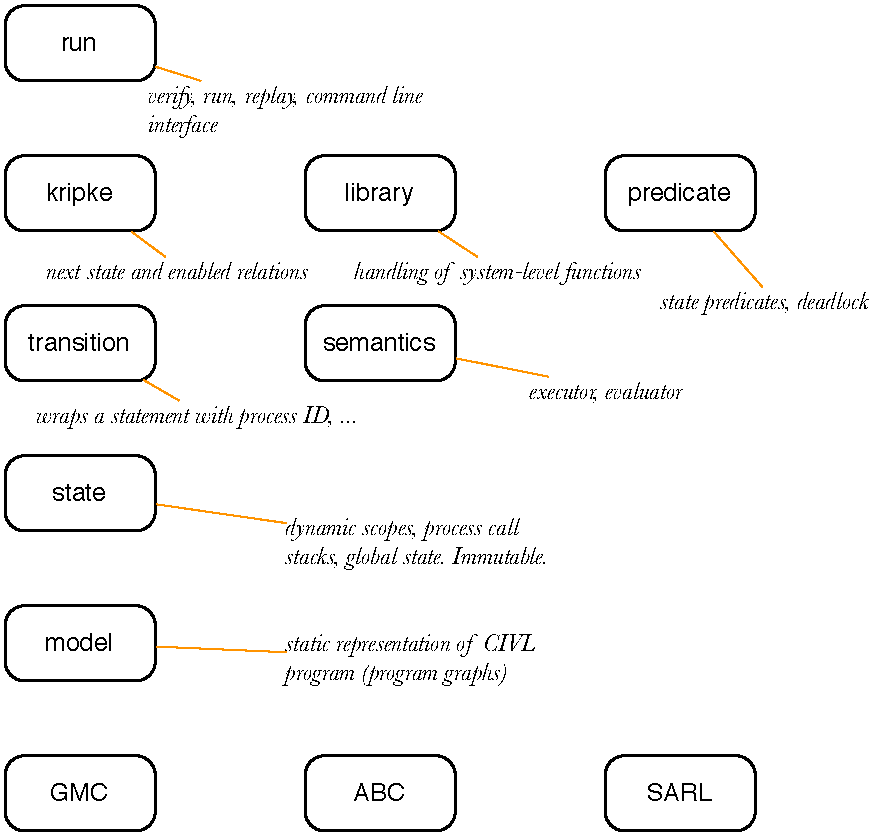
\includegraphics[scale=0.55]{civlModules}
    &
    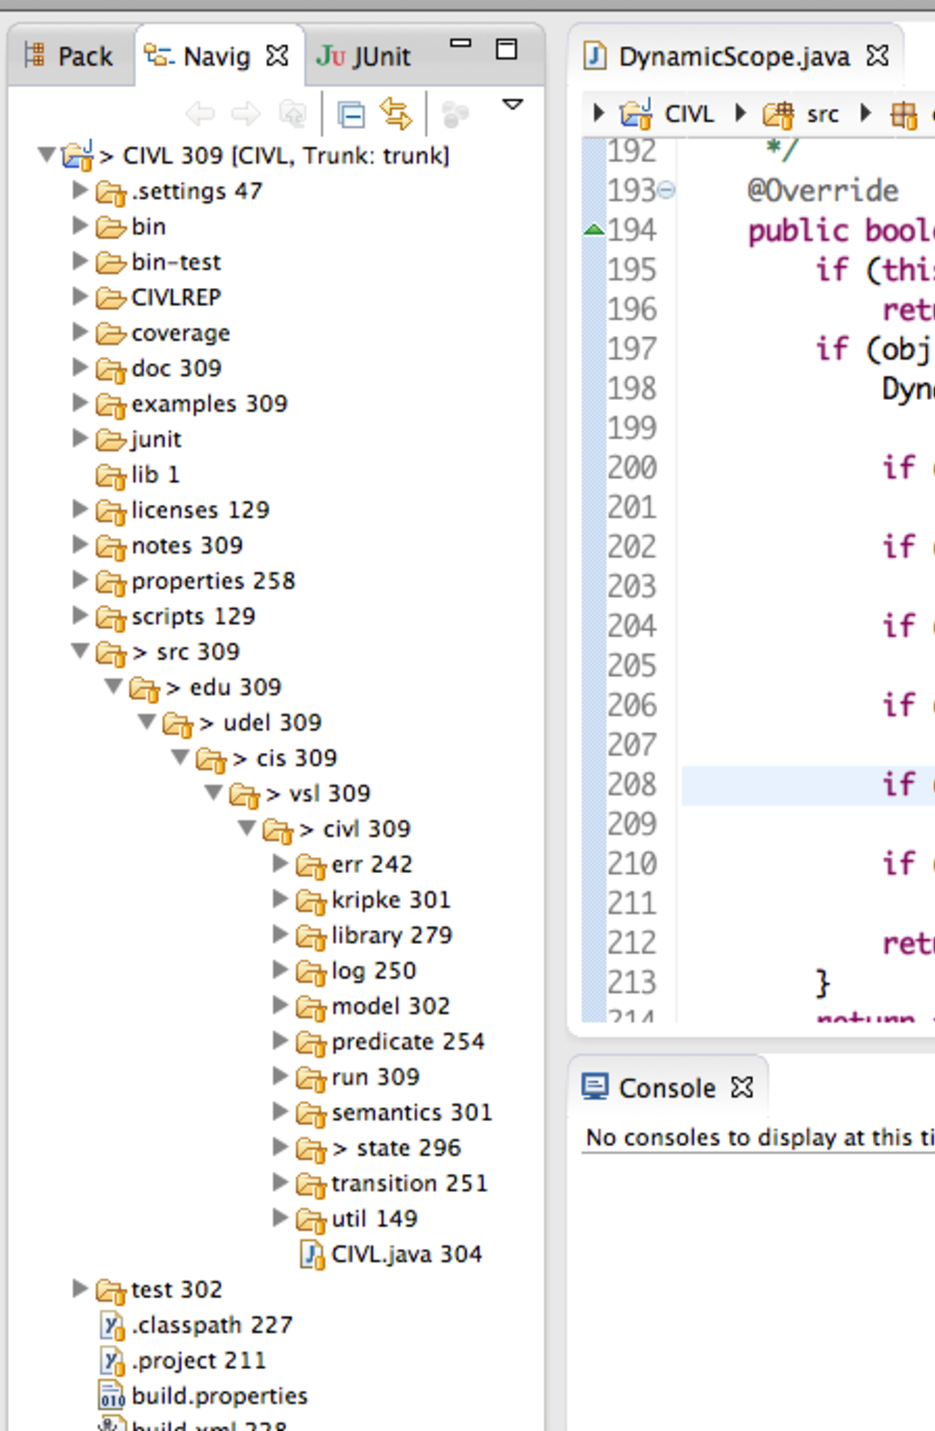
\includegraphics[scale=.3]{civlEclipseModules}
  \end{tabular}
\end{frame}

\end{document}
